\documentclass[conference,compsoc]{IEEEtran}
\usepackage{graphicx}
\usepackage[table]{xcolor}

\usepackage{datetime}

% *** CITATION PACKAGES ***
%
\ifCLASSOPTIONcompsoc
  % IEEE Computer Society needs nocompress option
  % requires cite.sty v4.0 or later (November 2003)
  \usepackage[nocompress]{cite}
\else
  % normal IEEE
  \usepackage{cite} 
\fi 
% cite.sty was written by Donald Arseneau
% V1.6 and later of IEEEtran pre-defines the format of the cite.sty package
% \cite{} output to follow that of the IEEE. Loading the cite package will
% result in citation numbers being automatically sorted and properly
% "compressed/ranged". e.g., [1], [9], [2], [7], [5], [6] without using
% cite.sty will become [1], [2], [5]--[7], [9] using cite.sty. cite.sty's
% \cite will automatically add leading space, if needed. Use cite.sty's
% noadjust option (cite.sty V3.8 and later) if you want to turn this off
% such as if a citation ever needs to be enclosed in parenthesis.
% cite.sty is already installed on most LaTeX systems. Be sure and use
% version 5.0 (2009-03-20) and later if using hyperref.sty.
% The latest version can be obtained at:
% http://www.ctan.org/pkg/cite
% The documentation is contained in the cite.sty file itself.
%
% Note that some packages require special options to format as the Computer
% Society requires. In particular, Computer Society  papers do not use
% compressed citation ranges as is done in typical IEEE papers
% (e.g., [1]-[4]). Instead, they list every citation separately in order
% (e.g., [1], [2], [3], [4]). To get the latter we need to load the cite
% package with the nocompress option which is supported by cite.sty v4.0
% and later.

% *** GRAPHICS RELATED PACKAGES ***
%
\ifCLASSINFOpdf
  % \usepackage[pdftex]{graphicx}
  % declare the path(s) where your graphic files are
  % \graphicspath{{../pdf/}{../jpeg/}}
  % and their extensions so you won't have to specify these with
  % every instance of \includegraphics
  % \DeclareGraphicsExtensions{.pdf,.jpeg,.png}
\else
  % or other class option (dvipsone, dvipdf, if not using dvips). graphicx
  % will default to the driver specified in the system graphics.cfg if no
  % driver is specified.
  % \usepackage[dvips]{graphicx}
  % declare the path(s) where your graphic files are
  % \graphicspath{{../eps/}}
  % and their extensions so you won't have to specify these with
  % every instance of \includegraphics
  % \DeclareGraphicsExtensions{.eps}
\fi
% graphicx was written by David Carlisle and Sebastian Rahtz. It is
% required if you want graphics, photos, etc. graphicx.sty is already
% installed on most LaTeX systems. The latest version and documentation
% can be obtained at: 
% http://www.ctan.org/pkg/graphicx
% Another good source of documentation is "Using Imported Graphics in
% LaTeX2e" by Keith Reckdahl which can be found at:
% http://www.ctan.org/pkg/epslatex
%
% latex, and pdflatex in dvi mode, support graphics in encapsulated
% postscript (.eps) format. pdflatex in pdf mode supports graphics
% in .pdf, .jpeg, .png and .mps (metapost) formats. Users should ensure
% that all non-photo figures use a vector format (.eps, .pdf, .mps) and
% not a bitmapped formats (.jpeg, .png). The IEEE frowns on bitmapped formats
% which can result in "jaggedy"/blurry rendering of lines and letters as
% well as large increases in file sizes.
%
% You can find documentation about the pdfTeX application at:
% http://www.tug.org/applications/pdftex


% *** MATH PACKAGES ***
%
%\usepackage{amsmath}
% A popular package from the American Mathematical Society that provides
% many useful and powerful commands for dealing with mathematics.
%
% Note that the amsmath package sets \interdisplaylinepenalty to 10000
% thus preventing page breaks from occurring within multiline equations. Use:
%\interdisplaylinepenalty=2500
% after loading amsmath to restore such page breaks as IEEEtran.cls normally
% does. amsmath.sty is already installed on most LaTeX systems. The latest
% version and documentation can be obtained at:
% http://www.ctan.org/pkg/amsmath

% *** SPECIALIZED LIST PACKAGES ***
%
%\usepackage{algorithmic}
% algorithmic.sty was written by Peter Williams and Rogerio Brito.
% This package provides an algorithmic environment fo describing algorithms.
% You can use the algorithmic environment in-text or within a figure
% environment to provide for a floating algorithm. Do NOT use the algorithm
% floating environment provided by algorithm.sty (by the same authors) or
% algorithm2e.sty (by Christophe Fiorio) as the IEEE does not use dedicated
% algorithm float types and packages that provide these will not provide
% correct IEEE style captions. The latest version and documentation of
% algorithmic.sty can be obtained at:
% http://www.ctan.org/pkg/algorithms
% Also of interest may be the (relatively newer and more customizable)
% algorithmicx.sty package by Szasz Janos:
% http://www.ctan.org/pkg/algorithmicx


% *** ALIGNMENT PACKAGES ***
%
%\usepackage{array}
% Frank Mittelbach's and David Carlisle's array.sty patches and improves
% the standard LaTeX2e array and tabular environments to provide better
% appearance and additional user controls. As the default LaTeX2e table
% generation code is lacking to the point of almost being broken with
% respect to the quality of the end results, all users are strongly
% advised to use an enhanced (at the very least that provided by array.sty)
% set of table tools. array.sty is already installed on most systems. The
% latest version and documentation can be obtained at:
% http://www.ctan.org/pkg/array

% IEEEtran contains the IEEEeqnarray family of commands that can be used to
% generate multiline equations as well as matrices, tables, etc., of high
% quality.

% *** SUBFIGURE PACKAGES ***
%\ifCLASSOPTIONcompsoc
%  \usepackage[caption=false,font=footnotesize,labelfont=sf,textfont=sf]{subfig}
%\else
%  \usepackage[caption=false,font=footnotesize]{subfig}
%\fi
% subfig.sty, written by Steven Douglas Cochran, is the modern replacement
% for subfigure.sty, the latter of which is no longer maintained and is
% incompatible with some LaTeX packages including fixltx2e. However,
% subfig.sty requires and automatically loads Axel Sommerfeldt's caption.sty
% which will override IEEEtran.cls' handling of captions and this will result
% in non-IEEE style figure/table captions. To prevent this problem, be sure
% and invoke subfig.sty's "caption=false" package option (available since
% subfig.sty version 1.3, 2005/06/28) as this is will preserve IEEEtran.cls
% handling of captions.
% Note that the Computer Society format requires a sans serif font rather
% than the serif font used in traditional IEEE formatting and thus the need
% to invoke different subfig.sty package options depending on whether
% compsoc mode has been enabled.
%
% The latest version and documentation of subfig.sty can be obtained at:
% http://www.ctan.org/pkg/subfig

% *** FLOAT PACKAGES ***
%
%\usepackage{fixltx2e}
% fixltx2e, the successor to the earlier fix2col.sty, was written by
% Frank Mittelbach and David Carlisle. This package corrects a few problems
% in the LaTeX2e kernel, the most notable of which is that in current
% LaTeX2e releases, the ordering of single and double column floats is not
% guaranteed to be preserved. Thus, an unpatched LaTeX2e can allow a
% single column figure to be placed prior to an earlier double column
% figure.
% Be aware that LaTeX2e kernels dated 2015 and later have fixltx2e.sty's
% corrections already built into the system in which case a warning will
% be issued if an attempt is made to load fixltx2e.sty as it is no longer
% needed.
% The latest version and documentation can be found at:
% http://www.ctan.org/pkg/fixltx2e

%\usepackage{stfloats}
% stfloats.sty was written by Sigitas Tolusis. This package gives LaTeX2e
% the ability to do double column floats at the bottom of the page as well
% as the top. (e.g., "\begin{figure*}[!b]" is not normally possible in
% LaTeX2e). It also provides a command:
%\fnbelowfloat
% to enable the placement of footnotes below bottom floats (the standard
% LaTeX2e kernel puts them above bottom floats). This is an invasive package
% which rewrites many portions of the LaTeX2e float routines. It may not work
% with other packages that modify the LaTeX2e float routines. The latest
% version and documentation can be obtained at:
% http://www.ctan.org/pkg/stfloats
% Do not use the stfloats baselinefloat ability as the IEEE does not allow
% \baselineskip to stretch. Authors submitting work to the IEEE should note
% that the IEEE rarely uses double column equations and that authors should try
% to avoid such use. Do not be tempted to use the cuted.sty or midfloat.sty
% packages (also by Sigitas Tolusis) as the IEEE does not format its papers in
% such ways.
% Do not attempt to use stfloats with fixltx2e as they are incompatible.
% Instead, use Morten Hogholm'a dblfloatfix which combines the features
% of both fixltx2e and stfloats:
%
% \usepackage{dblfloatfix}
% The latest version can be found at:
% http://www.ctan.org/pkg/dblfloatfix

% *** PDF, URL AND HYPERLINK PACKAGES ***
%
%\usepackage{url}
% url.sty was written by Donald Arseneau. It provides better support for
% handling and breaking URLs. url.sty is already installed on most LaTeX
% systems. The latest version and documentation can be obtained at:
% http://www.ctan.org/pkg/url
% Basically, \url{my_url_here}.

% *** Do not adjust lengths that control margins, column widths, etc. ***
% *** Do not use packages that alter fonts (such as pslatex).         ***
% There should be no need to do such things with IEEEtran.cls V1.6 and later.
% (Unless specifically asked to do so by the journal or conference you plan
% to submit to, of course. )

% correct bad hyphenation here
\hyphenation{op-tical net-works semi-conduc-tor}
   
\usepackage{hyperref}
 
\begin{document}
% 
% paper title
% Titles are generally capitalized except for words such as a, an, and, as,
% at, but, by, for, in, nor, of, on, or, the, to and up, which are usually
% not capitalized unless they are the first or last word of the title.
% Linebreaks \\ can be used within to get better formatting as desired.
% Do not put math or special symbols in the title.
\title{Enigma Machine: an encryption device capable of decryption simultaneously\\
{\small \today~-~\currenttime}}

 
% author names and affiliations
% use a multiple column layout for up to three different
% affiliations
\author{\IEEEauthorblockN{Adel Dedic}
\IEEEauthorblockA{University of Luxembourg\\
Email: adel.dedic.001@student.uni.lu}
\\
{\bf This report has been produced under the supervision of:}\\
\IEEEauthorblockN{Benoît Ries}
\IEEEauthorblockA{University of Luxembourg\\
Email: benoit.ries@uni.lu}%
}

% conference papers do not typically use \thanks and this command
% is locked out in conference mode. If really needed, such as for
% the acknowledgment of grants, issue a \IEEEoverridecommandlockouts
% after \documentclass

% for over three affiliations, or if they all won't fit within the width
% of the page (and note that there is less available width in this regard for
% compsoc conferences compared to traditional conferences), use this
% alternative format:
% 
%\author{\IEEEauthorblockN{Michael Shell\IEEEauthorrefmark{1},
%Homer Simpson\IEEEauthorrefmark{2},
%James Kirk\IEEEauthorrefmark{3}, 
%Montgomery Scott\IEEEauthorrefmark{3} and
%Eldon Tyrell\IEEEauthorrefmark{4}}
%\IEEEauthorblockA{\IEEEauthorrefmark{1}School of Electrical and Computer Engineering\\
%Georgia Institute of Technology,
%Atlanta, Georgia 30332--0250\\ Email: see http://www.michaelshell.org/contact.html}
%\IEEEauthorblockA{\IEEEauthorrefmark{2}Twentieth Century Fox, Springfield, USA\\
%Email: homer@thesimpsons.com}
%\IEEEauthorblockA{\IEEEauthorrefmark{3}Starfleet Academy, San Francisco, California 96678-2391\\
%Telephone: (800) 555--1212, Fax: (888) 555--1212}
%\IEEEauthorblockA{\IEEEauthorrefmark{4}Tyrell Inc., 123 Replicant Street, Los Angeles, California 90210--4321}}




% use for special paper notices
%\IEEEspecialpapernotice{(Invited Paper)}




% make the title area
\maketitle

%to remove for your report
%\footnote{}

% As a general rule, do not put math, special symbols or citations
% in the abstract
\begin{abstract}
This  document  is  the  final  report  of  the  Bachelor Semester   Project   of   the   student   Adel Dedic   which   was conducted with the help of his tutor Benoît Ries. This project is  part  of  the  Bachelor  in  Computer  Science  program  at  the University of Luxembourg during the first semester of study. This project is looking to produce a program that is reminiscent to the original Enigma machine. With the assistance of distinct flaws that surround the Enigma, the security of the machine is examined and thus prompting another option for communication.

\end{abstract}

% no keywords

% For peer review papers, you can put extra information on the cover
% page as needed:
% \ifCLASSOPTIONpeerreview
% \begin{center} \bfseries EDICS Category: 3-BBND \end{center}
% \fi
%
% For peerreview papers, this IEEEtran command inserts a page break and
% creates the second title. It will be ignored for other modes.
\IEEEpeerreviewmaketitle

\section{Introduction}
% no \IEEEPARstart
An encryption system that was invented during the most frightful years for somebody to endure has took many by surprise by how difficult it is to break, considered impossible to crack during it's time, with such a sophisticated machinery that little of few people knew how it works even less so how to build one of their own.\\
One of the first Enigma patent was filed in 1918 by co-founders of a German firm, Scherbius and Ritter, for it's sole purpose being an option for communication for companies and governments that is safe and well protected against outside intervention. During it's time, no body knew how important of an object such as Enigma would be crucial for the outcome of World War II.\\
The main scientific objective of the Bachelor Semester Project is to analyse the strength of Enigma and conclude if the device could be considered as an alternative to safe communication. Different aspects of the machine are examined to further highlight the strengths and weaknesses of the machine.\\
The main technical objective of the BSP will be to create a program that should simulate the intentions of the original Enigma machine, that being able to encrypt and decrypt messages simultaneously in one piece of software.
Other prominent features like how the encryption part behaves where every character is encrypted dynamically but also the possibility of configuring the rotors are all present. The program is equipped with features that eases the usability like being able to export and import keys that contain only the crucial information for being processed and thus making the program imminent for being able to read the contents of the key file.\\


\section{Project description}
\subsection{Domains}
\subsubsection{Scientific }
In the scientific part of this project will cover articles which are related to security in general and the diverse types of encryption. The different types of cryptography are relevant to the project by being a solution of some sort to one of the main issues that Enigma has.\\
Analysing and researching security breaches of Enigma is our main domain of the project.\\
Furthermore, we will analyse how the mathematicians had broken the Enigma by using another fundamental feature of the machine and explain in fact the whole process of encryption works in that case.\\

\subsubsection{Technical}
In the technical part of this project a program is produced that simulates the Enigma machine. A GUI for the program is developed to compliment the original piece (e.g.: visual rotor settings). The main domain used to produce the technical was a programming language called Python. One of the main reasons why Python was used was solely based upon the fact that this programming language promotes readability and it is well suited for small and large scale projects like this.\\

\subsection{Targeted Deliverables}
\label{sec-deliverables}
\subsubsection{Scientific deliverables}
As a scientific report, some research is required to understand where the breaking points of the original Enigma are laid but also in the regard of the breaking point a remediation is proposed that could be implemented to modernize the machine. Once these are explained a small somewhat conclusion is presented to provide a scientific explanation for how these are related to the security of the Enigma.

\subsubsection{Technical deliverables}
As a technical report a program will be developed to simulate the original Enigma machine that is equipped with the option of encryption and decryption following the rotors settings that have been configured previously. The software is developed through Python thus is lightweight but also no other external software is required to work. \\
The option to export a key is also provided to make the exchange of messages more user friendly but the key solely is useless without the software due to the fact only crucial information is saved upon. Furthermore, a Graphical User Interface is created following a distinct homage to the original machine.\\


% \subsection{Constraints}
% Provide all the constraints that were to be considered for the project.
% A constraint is a property that is agreed by you and your PAT to have been satisfied before starting the project.
% An example could be ``good level in Python programming''. 
% As a consequence the work done to satisfy the constraints cannot be presented as a deliverable of the BSP.

\section{Pre-requisites}

\subsection{Scientific pre-requisites}
To successfully understand the scientific report, no actual pre-requisite was necessary.
But something that was useful to comprehend is simple knowledge of comparison.
\subsection{Technical pre-requisites}
The technical part of the BSP is coded in Python, thereby knowledge about coding in Python is recommended.\\
This applies to any general programming knowledge as well not necessarily Python only.\\
Taken in consideration that not all programming languages share same structure or functions.\\


\section{ Security of Enigma}
\label{sec-production}
\subsection{Requirements}
The purpose of the deliverable is to research and formalize an answer to the following question: \emph{How secure is Enigma ?}\\
Therefore, the deliverable shall cover:
\begin{itemize}
    \item{[4.3.1.]} Describing what Enigma is
    \item{[4.3.2.]} Analysing the value of combinations
    \item{[4.3.3.]} Defining the word 'encryption' and how it works in the case of Enigma
    \item{[4.3.4.]} Defining what a breaking point in the context means
    \item{[4.3.5.]} Explaining Breaking Point N°1: Key Exchange
    \item{[4.3.6.]} Explaining Breaking Point N°2: Fundamental encryption problem which refuses to let a letter to be encoded into itself during the encryption process
    \item{[4.3.7.]} Summarizing the relation between the breaking points and the security of the Enigma
\end{itemize}

\subsection{Design}
The scientific deliverable shall explain through a brief description of what Enigma is and introduce encryption which is also further explained at a later point. Another aspect which will be brought up is the analysis of how many different combinations the military version of Enigma is capable to be configured in. This will explain the reason why it was that much harder for code-breakers at the time to even come close at 'cracking' the code in time before the message became obsolete.\\
With that out of the way, the main part of the report is to explain the flaws of Enigma, in this case we call them 'breaking points' and shall be respectfully defined before any examples are given, and present a remedy for each flaw.\\

The first flaw "Key exchange" was of a lesser problem back in the day but to today's standards is as important as the cipher itself. Thereby some examples of today's implementation for key exchange is presented.\\
The examples provided come from an article from Wikiwand called "Key exchange", these examples are one of many different ways of improving key distribution concerning of modernizing Enigma machine.\\ 

The second flaw, was more focused on the functionality of how encryption behaves concerning Enigma and explain how this affects the security thereby how it could be used to break it.\\
To illustrate a concrete example, a similar approach as the one in an article from Brilliant: "Enigma Machine - Cracking the Enigma Code" was used to explain.\\

As a final touch, the points of failure of Enigma and also the complexity will be taken in consideration to produce an answer if the Enigma is well suited and secure enough for the intended use.\\

\subsection{Production}

The production is produced following specific steps of defining the important nouns that are going to be used, by using the various resources each breaking point is talked extensively and finally the conclusion at the end is representing the relation between the flaws of the Enigma with it's security.\\  

\subsubsection{Enigma} Enigma is an encryption device which was mostly used by the Germans during the WWII, it was capable of configuring trillions of combinations and thereby rendering the cipher \underline{almost} impossible to crack and such it was preferred way for German army to communicate due being believed at the time that the machine was unbreakable.\\
The way it worked it was by permuting each letter into another one with the help of rotors and other components like the plugboard and the reflector. In this case, the rotors act like a step for the letter to move and the rotors change dynamically each time a letter is pressed. As soon as one rotor finishes the whole turn, the second rotor next to it will turn by 1 and so-on.\\

\subsubsection{Number of combinations}
As stated above, it was believed by the Germans with confidence that the machine was unbreakable and it wasn't without their reasons. To explain, I will take in consideration of the early models of Enigma that was using by the German army, Funkschlüssel C ("Radio cipher C").\\
This model had introduced the plugboard to the mix of combinations but also giving the option to choose 3 out of 5 different rotors whose order in which placed matters.\\
\begin{equation}
    \frac{5!}{5-3!}=60
\end{equation}
For the 3 out of 5 rotors, the order can be arranged in 60 ways.\\

\begin{equation}
    26^3=17576
\end{equation}
Each of the 3 rotors have 26 possible positions making another 17 576 ways to configure.\\
\begin{equation}
    \frac{26!}{(26-20)!\times2^{10}\times10!}=150738274937250
\end{equation}
And lastly the plugboard with 10 different pairs of letters being to switched, with the greatest impact, it allows another 150 738 274 937 250 of different combinations.\\
If we multiply these factors we end up with 158 962 555 217 826 360 000 (almost 159 quintillion) possible combinations that the machine is able to be set in. And considering the fact that at the time all of the combinations were tested out manually by hand, it's not surprising why it was believed that nobody could crack the Enigma.\\
If somebody would try to go over every possible combination and managed to keep a speed of trying one combination a second, it would still take at least a bit over than 5 trillion years to go through each configuration one by one. ($\frac{158962555217826360000}{60\times60\times24\times365.5}\approx5.034\times10^{12}$)

\subsubsection{Encryption} Encryption is another means of securing information with a help of mathematical techniques and algorithms. Usually a key is provided which is used to access the information back. The encryption process offers information unreadable to anybody without the proper key. This technique of securing information is advantageous fighting off hackers who are willing to access sensitive information.\\

\subsubsection{Breaking Points} To continue forward we will have to define what a breaking point in this case is standing for. Each machine of technology is undoubtedly made by a human hand and thereby the chances of a machine to be flawed is greater than expected due to the nature of humans being flawed as well. A breaking point is a feature of the machine which was left for outside intervention to fiddle with and exploiting other property of the machine. In this case, each breaking point is a vulnerability that anybody can use to achieve accessing the hidden meaning behind an encrypted message.\\

\subsubsection{Breaking Point N°1: Key Exchange} Each encryption method is conventionally accompanied by a key that is used to process the information encrypted readable again. And thus, for an encryption method to be reliable security of the key plays a big role. At the beginning, people relied on confidentiality of securing the key and utilized a single key thereby the method was called 'single-key' cryptography.\\
'Single-Key' cryptography (also called 'symmetric encryption') in fact provided insecurities on the level where if the two parties failed exchanging properly the key it increased the chance for a third party to gain acquisition of the key.\\
Thereby, another methods have been introduced, specifically a two-key system which was the famous 'public-key' cryptography (also called 'asymmetric encryption').\\
It was accompanied with a private and a public key, based on what encryption algorithms was used the uses of these keys depended on it. i.e.: 'Rivest-Shamir-Adleman' (RSA) used the private key for decryption of information where as 'Digital Signature Algorithm' (DSA) used it for authentication purposes.\\
Another method of securely exchanging keys is the famous 'Diffie-Hellman' (DH) method, even though this method was one of the earliest to come to light it's still broadly used on multiple platforms. The method consists of generating a unique public and a unique private key for both parties resulting a combination of one's private key and other's public key gives out the secret information.\\
For a clearer picture, an example from an article is shown as Figure \ref{fig:dh}.\\
Enigma on the other hand didn't follow any of these 'modern' methods of key exchange and would simply share list of day-to-day configurations of the Enigma to trusted parties which would not be changed for a whole month. These configurations can be considered as a 'key' in modern day cryptography.
To today's standards, this in fact is very dangerous way of distributing information because if it would land on the wrong hands the leak of information wouldn't be resolved soon enough to prevent drawbacks. (In the case of Enigma, war obstructions)\\ 
Nonetheless, in this case a simple solution is to modernize the key distribution by using more modern methods like stated above (i.e.:  RSA, DSA, DH, \ldots)

\subsubsection{Breaking Point N°2: Fundamental encryption problem}
During the WWII, many of the parties that were trying to break Enigma have noticed a simple but very big failure in the encryption technique of the machine. Which was too difficult to fix provided by the techniques that existed at the time. The flaw was lying much deeper under the surface and involved many interactions between other components to resolve.
This was due to the fact that all of the components of the machine worked mechanically between each other and if anybody would dare to handle it issues would occur making it unreliable to be used at the time.\\
e.g.: if the 'pathway' is disrupted or overlapped a short-circuit would take place (Please see Figure \ref{fig:path} to observe the functionality of the pathway)\\
Thereby, another breaking point of Enigma was the fact that a letter cannot represent itself during encryption based on the functionality.\\
Which means, when the user would press the letter "A", the output would \underline{never} be encoded as the letter "A".\\
When a letter is pressed on the machine, an electrical flow is created which passes through numerous components that help permute the letter, in this case rotors and the reflector.
The electrical flow follows an unique 'pathway' from the pressed letter and lightened up letter. The path never intersects thus the electrical flow can never arrive to the same position where it departed from.\\
This information was a great deal for mathematicians and code-breakers at the time, because it gave them a hint and something to work on because previously they've been working blindly on how to break the Enigma.\\
At this point, since they knew about the flaw they were missing only one element to pursue and that was to guess a word which would always be included into the enciphered messages. In this case, they found out that a weather report and the phrase "Heil Hitler" was always included, where the latter was at the end of a letter and former at the beginning.\\
With these two elements, mathematicians used a specific method to break the code; the method was 'process of elimination'. They would compare words to the letters of the code and in the case where a single letter from word was also in the code, then they were assured that the word is not part of the code based on the fact that a letter cannot be itself.\\

To further explain how this affects the functionality of the machine, we will provide an example* which will be color indicated; red meaning the two letters overlap and green meaning that they don't.\\
Let's suppose we're comparing the word "windy" to the code (The symbol \# is to indicate the unknown letters):\\

\begin{tabular}{ |c|c|c|c|c|c|c|c|c| }
 \hline
 Coded Message & \cellcolor{red!35}W & S & I & T & V & N & A \\ 
 \hline
 Word & \cellcolor{red!35}W & \cellcolor{green!35}I & \cellcolor{green!35}N & \cellcolor{green!35}D & \cellcolor{green!35}Y & \# & \# \\
 \hline
\end{tabular}\\

Since the letter 'W' are matching up, means that this doesn't hold up.\\

\begin{tabular}{ |c|c|c|c|c|c|c|c|c| }
 \hline
 Coded Message & W & S & \cellcolor{red!35}I & T & V & N & A \\ 
 \hline
 Word & \# & \cellcolor{green!35}W & \cellcolor{red!35}I & \cellcolor{green!35}N & \cellcolor{green!35}D & \cellcolor{green!35}Y & \# \\
 \hline
\end{tabular}\\

In this case the letter 'I' is matching, thereby also not the right encoding.\\

\begin{tabular}{ |c|c|c|c|c|c|c|c|c| }
 \hline
 Coded Message & W & S & I & T & V & N & A \\ 
 \hline
 Word & \# & \# & \cellcolor{green!35}W & \cellcolor{green!35}I & \cellcolor{green!35}N & \cellcolor{green!35}D & \cellcolor{green!35}Y \\
 \hline
\end{tabular}\\

%\begin{verbatim}
%console.log("test")
%\end{verbatim}

In the last case none of the letters match up, which means that the encoding works in this case. Take in consideration that the word 'Windy' isn't guaranteed that it is in the secret message itself but it gives us a bigger picture understanding where to start looking for breaking messages.\\

In conclusion, the elementary solution is to provide a possibility for the machine to be able to encrypt letters into themselves. This in fact would eliminate the current method of breaking the code and thereby increase the security of the device immensely.\\

\subsubsection{Relation between breaking points \& security} Considering the fact that all of the breaking points have been covered by now, to complete the scientific report we shall answer the question that has been asked at the beginning \emph{"How secure is Enigma ?"}\\

Without any improvements to the original Enigma, it's sufficiently secure for personal uses between two parties due the examination of the sheer value of possible combinations that the machine can be set up, but if the intent is to use the machine on a larger scale like business organizations then the breaking points should be taken in consideration and implement the remedies that have been listed. Especially because nowadays a computer is much faster than a human and the 5 trillions of years that a human would take to break it, a sufficiently strong enough processor from a modern computer can examine all of the combinations under 2 minutes confidently.\\
Thereby to ensure more security we should firstly improve the way to exchange the key more securely by using better methods of key exchange like the Diffie-Hellman method and secondly eliminate the possibility of exploiting the not-intended feature where a key can not be encoded into itself.\\




\subsection{Assessment}
The scientific deliverable established the flaws of Enigma and through research, some examples have been provided on how to fix those issues. Furthermore, we present two cases for one which the original Enigma without any modifications is very well suitable for personal use but for the other case, where security is a bigger issue of importance, to take in consideration the modify the machine following the recommendation that was given to ensure a safer broad communication between two parties.\\
Thereby, we have successfully presented how secure Enigma is and what precautions we can still take to improve its security.\\

\section{Program: Enigma Simulator}
\label{sec-production}

\subsection{Requirements}
The program is supposed to polished and posses similarities but also improve upon if necessary the original Enigma machine, in this case:
\begin{itemize}
    \item The program should include an interface that reassemble the original
    \item Fully configurable rotor settings which would increment dynamically in a respectful order (first rotor 1 then rotor 2 and so-on)
    \item Unlike the original, a text-box where the user is able to input a whole string of text and process it whole thanks to a simple button
    \item The program shall output enciphered string of text which was processed through the following rotor settings as configured
    \item The program shall provide functionality of importing and exporting 'keys'
    \item For usability, the user shall be able to test strings by quickly transferring output to input
    \item The program shall still remain user-friendly
    \item And finally, the program shouldn't depend on anything external to function alike the original
\end{itemize}

\subsection{Design}
The program is easily readable from the surface as soon as the user is introduced to it; on the top the 'rotor section' is located where the user is supposed to insert his/her set of rotor settings. To confirm the rotors, the user shall press the 'Set' button to finalize the process.\\
This is the first thing the user should be introduced to because this the main functionality of the program and the configuration chosen represents the unique key in that instance for the processed message. The configured settings are important to remember, without them the original message cannot be retrieved as easily. Thereby, when the user has set them, the rotors settings are visible to the user thanks to the message above where it clearly states the rotor settings in the form of (X/X/X) where 'X' designates the value of the rotor in the respectful order.\\

Furthermore, the section right below the rotors is where the 'input section' is located. This is where the user is supposed to insert a string of text, that being a simple phrase or a whole paragraph of text, which he/she is wishing to process.\\

Moreover, the similar section right after is where the 'output section' is located. This section is nothing to be mangled with as it only provides an output through the functions of buttons and doesn't provide anything except that.\\

The reason for inclusion of the last two mentioned sections is to provide usability to the user, unlike the original Enigma machine the user was supposed to type each letter through key-by-key method and would result into a annoying pattern where if the user somehow messes up, he's supposed to start all over again. With the inclusion of the 'input section', the user can easily import a whole string of text and process it whole while still following the procedures of dynamic rotors in the back-end and output the whole result in the 'output section' and thereby eliminate any frustration which was known to exist with the original Enigma machine.\\

Finally the given buttons at the end are self-explanatory by their name. i.e.: 'Transfer','Encrypt', 'Decrypt', 'Export*' and 'Import*'\\
A notice is provided to explain that the 'Export*' and 'Import*' buttons function in aid of a text file specifically named 'key.txt' file.\\

The practicality of these buttons extends greater than what it represents on the surface. 'Transfer' button exists due to the reasons if the user is willing to test quickly some length of strings and be provided of what the result may be.\\

'Encrypt' and 'Decrypt' are designated for flexibility of the program as it adds upon options to the user, these in fact are very necessary because they include the main objectives of the program itself. Unlike the original where a mechanical 'pathway' is created each time a key is pressed, that 'pathway' doesn't exist in the case of this program due it to not being necessary to properly function and also in this case the user has options to decide how exact he/she wants it to behave like.\\

The buttons 'Export*' and 'Import*' are again an addition that provide an ease of functionality where the user isn't supposed to write enciphered messages and accompanied rotor configurations manually. The buttons read/create files which include important information (rotor settings and the processed message) and implement them accordingly. In the case of 'Import*', the rotor settings is set and the message is imported into the 'input section' and enables the function to 'Decrypt' the message for the user. On the other hand, the 'Export*' saves the message and settings onto a text-file named 'key.txt'.\\

The 'key.txt' file created upon 'Export' is easily readable by a human but the contents of the communication cannot be fully understood without the program to decrypt the processed message.\\ 

\subsection{Production}

The functionalities that were present in the original Enigma machine were all separated and developed into functions in a python programming language.\\
First being the 'rotate character' whose job is to permute a character by a step where the step in this case is a permutation of the rotors.\\
If for any case an interpretation is necessary, please take a look at the last Figure \ref{fig:infac} where the whole interface of the software is presented.\\

This is a sneak peek of how the 'step' that is necessary for encryption is permuted
\begin{verbatim}
        c_num += enigma.rotor1
        c_num -= enigma.rotor2
        c_num += enigma.rotor3*2
        c_num %= window_width
\end{verbatim} 
The permutation is a process of 4 different mathematical operations:\\
\begin{itemize}
    \item Firstly adding the rotor 1 to the step;\\
    \item Secondly subtracting the rotor 2 from the step;\\
    \item Thirdly, adding the double of the rotor 3 to the step.\\
    \item Finally, as we want to keep the step between the borders of letters in the alphabet (1-26), we perform a operation that assures us that result because the first 3 permutations may end up with a step greater than 26.\\
\end{itemize}

The stated mathematical operations are produced in a way to result a non-commutable rotors behaviour. This means that the order the user has set them up plays a big role into securing the code and thus making it harder to break but also creates a configuration which is unique.\\ 
For the operations themselves are designed to produce a more linear 'step' and balancing how far the 'step' can go in either direction. Increasing or making the operations harder to compute does not have a greater expense on the security due to how the encryption can behave.\\
e.g. The alphabet is consisted of 26 letters and thus if the 'step' is much greater ($>$100) will only turn around but still end-up between 1 and 26 (which are designated for each letter of the alphabet).\\

Second part is the 'rotor change' whose objective is to increment rotors in a respectful order and make sure that the rotors stay between their boundaries (1-26).\\
This means that through many 'if statements' we assure that rotors behave like they're supposed to.\\
Once the first rotor completes a whole turn the second rotor increments by 1 and so on.\\
This is carefully made to resemble the functionality of the original version of Enigma because the original rotor was also bounded between the values of 1 to 26.\\

Third part which in this case is two different functions, those being 'encrypt' and 'decrypt'. The prior being the main function whose objective is to rotate (encrypt) each character while also initiating the 'rotor change' each time. This provides a 'step' which in fact is dynamic in this case for each character of a given string.\\

The following is a preview of the main body for encryption method in the program:
\begin{verbatim}
    c = rotate_character(c, 'A', 'Z')
    c = rotate_character(c, 'a', 'z')
    c = rotate_character(c, '0', '9')
    result +=c
    rotor_change()
\end{verbatim}

For the decryption part, the same method is able to be called but we have to make sure that the steps taken are simply in the reversed position because we want to back track the steps taken previously during the encryption process.\\

The reason why there are two separate functions is due to the by-product of willing to present a more modern version of Enigma where the user is able to input a whole string of text and process them as a whole. The whole functionality is quite more satisfying as a result if compared to the old technique where each letter or character had to pressed in a key-by-key method.\\

For productivity, if the user desires to test strings out another choice is given in the middle of the interface called 'transfer'. It is carefully placed in between of the two text boxes to incentivize its functionality of being able to 'transfer' the given output as the input and thus the user is able to proceed processing the message again. This in fact results into a more fluent orientation through the program because it offers the user to test strings easier.  \\


Last part of the program is the functionality of import/export, whose job is create, respectfully read, a text file named 'key.txt'. The contents of the file created can be observed in the Figure \ref{fig:sample}.\\
It is well structured for the reasons if anybody is interested to access the file to observe. But as said before, the contents of the message can be seen but meaning behind it is inaccessible without the program to process it first.\\

The intention of all of the new additions compared to the original is to provide usability to the user but also adding a better user-friendly experience whilst operating with the program. The change to the interface compared to the original was quite needed as well to fulfill the intention of a more user-friendly interface and a way to incorporate all of the newly added features.\\
This version provides the user to process a whole string of a text instead of the 'key-by-key' method, due to the reason where latter provided a slow process to read longer texts but also has greater chance of blundering a letter which would require to restart the process of decryption because if by any mistake the user would press an incorrect letter the rotor would increment no matter what.\\

\subsection{Assessment}
As desired the product at the end is behaving very similarly to the original Enigma, from the feature of dynamic rotors to behaviour of encryption, the product is successfully accomplished.\\
The program is capable of encryption, decryption and saving keys in a easier fashion.\\
The product is user-friendly with a more modernized interface but still staying true to it's predecessors.\\
The interface has been clearly done to favor even those who don't know much about it Enigma. It promotes testing and playing around with each functionality.\\


\section*{Acknowledgment}
The author would like to personally thank the BiCS management, education team, his tutor Benoit Ries and his tutor's assistant Paul Houssel for the great help and time investment during the project. They helped to overcome any issue that had occurred during the journey.


\section{Conclusion}

This project helps understand how far the encryption methods have evolved and how much the techniques from the past became obsolete compared to the modern ones. Many new methods of key exchange have been created to provide a more tight communication between different parties and this project incorporates the new methods to provide an example for a more secure product.\\   
Furthermore, the program helped also understand how innovating the machine was for it's time and why it took so long for many people to break it.\\
Overall we are satisfied with the final deliverable and the product created can always be used to communicate anything discrete if needed.\\

\section{Plagiarism statement}

\newline
I declare that I am aware of the following facts:
\begin{itemize}
	\item As a student at the University of Luxembourg I must respect the rules of intellectual honesty, in particular not to resort to plagiarism, fraud or any other method that is illegal or contrary to scientific integrity.
	\item My report will be checked for plagiarism and if the plagiarism check is positive, an internal procedure will be started by my tutor. I am advised to request a pre-check by my tutor to avoid any issue.
	\item As declared in the assessment procedure of the University of Luxembourg, plagiarism is committed whenever the source of information used in an assignment, research report, paper or otherwise published/circulated piece of work is not properly acknowledged. In other words, plagiarism is the passing off as one’s own the words, ideas or work of another person, without attribution to the author. The omission of such proper acknowledgement amounts to claiming authorship for the work of another person. Plagiarism is committed regardless of the language of the original work used. Plagiarism can be deliberate or accidental.
Instances of plagiarism include, but are not limited to:
\begin{enumerate}
  \item Not putting quotation marks around a quote from another person’s work
  \item Pretending to paraphrase while in fact quoting
  \item Citing incorrectly or incompletely
  \item Failing to cite the source of a quoted or paraphrased work
  \item Copying/reproducing sections of another person’s work without acknowledging the source
  \item Paraphrasing another person’s work without acknowledging the source
  \item Having another person write/author a work for oneself and submitting/publishing it (with permission, with or without compensation) in one’s own name (‘ghost-writing’)
  \item Using another person’s unpublished work without attribution and permission (‘stealing’)
  \item Presenting a piece of work as one’s own that contains a high proportion of quoted/copied or paraphrased text (images, graphs, etc.), even if adequately referenced
\end{enumerate}
Auto- or self-plagiarism, that is the reproduction of (portions of a) text previously written by the author without citing that text, i.e. passing previously authored text as new, may be regarded as fraud if deemed sufficiently severe.
\end{itemize}

% An example of a floating figure using the graphicx package.
% Note that \label must occur AFTER (or within) \caption.
% For figures, \caption should occur after the \includegraphics.
% Note that IEEEtran v1.7 and later has special internal code that
% is designed to preserve the operation of \label within \caption
% even when the captionsoff option is in effect. However, because
% of issues like this, it may be the safest practice to put all your
% \label just after \caption rather than within \caption{}.
%
% Reminder: the "draftcls" or "draftclsnofoot", not "draft", class
% option should be used if it is desired that the figures are to be
% displayed while in draft mode.
%
%\begin{figure}[!t]
%\centering
%\includegraphics[width=2.5in]{myfigure}
% where an .eps filename suffix will be assumed under latex, 
% and a .pdf suffix will be assumed for pdflatex; or what has been declared
% via \DeclareGraphicsExtensions.
%\caption{Simulation results for the network.}
%\label{fig_sim}
%\end{figure}

% Note that the IEEE typically puts floats only at the top, even when this
% results in a large percentage of a column being occupied by floats.


% An example of a double column floating figure using two subfigures.
% (The subfig.sty package must be loaded for this to work.)
% The subfigure \label commands are set within each subfloat command,
% and the \label for the overall figure must come after \caption.
% \hfil is used as a separator to get equal spacing.
% Watch out that the combined width of all the subfigures on a 
% line do not exceed the text width or a line break will occur.
%
%\begin{figure*}[!t]
%\centering
%\subfloat[Case I]{\includegraphics[width=2.5in]{box}%
%\label{fig_first_case}}
%\hfil
%\subfloat[Case II]{\includegraphics[width=2.5in]{box}%
%\label{fig_second_case}}
%\caption{Simulation results for the network.}
%\label{fig_sim}
%\end{figure*}
%
% Note that often IEEE papers with subfigures do not employ subfigure
% captions (using the optional argument to \subfloat[]), but instead will
% reference/describe all of them (a), (b), etc., within the main caption.
% Be aware that for subfig.sty to generate the (a), (b), etc., subfigure
% labels, the optional argument to \subfloat must be present. If a
% subcaption is not desired, just leave its contents blank,
% e.g., \subfloat[].


% An example of a floating table. Note that, for IEEE style tables, the
% \caption command should come BEFORE the table and, given that table
% captions serve much like titles, are usually capitalized except for words
% such as a, an, and, as, at, but, by, for, in, nor, of, on, or, the, to
% and up, which are usually not capitalized unless they are the first or
% last word of the caption. Table text will default to \footnotesize as
% the IEEE normally uses this smaller font for tables.
% The \label must come after \caption as always.
%
%\begin{table}[!t]
%% increase table row spacing, adjust to taste
%\renewcommand{\arraystretch}{1.3}
% if using array.sty, it might be a good idea to tweak the value of
% \extrarowheight as needed to properly center the text within the cells
%\caption{An Example of a Table}
%\label{table_example}
%\centering
%% Some packages, such as MDW tools, offer better commands for making tables
%% than the plain LaTeX2e tabular which is used here.
%\begin{tabular}{|c||c|}
%\hline
%One & Two\\
%\hline
%Three & Four\\
%\hline
%\end{tabular}
%\end{table}


% Note that the IEEE does not put floats in the very first column
% - or typically anywhere on the first page for that matter. Also,
% in-text middle ("here") positioning is typically not used, but it
% is allowed and encouraged for Computer Society conferences (but
% not Computer Society journals). Most IEEE journals/conferences use
% top floats exclusively. 
% Note that, LaTeX2e, unlike IEEE journals/conferences, places
% footnotes above bottom floats. This can be corrected via the
% \fnbelowfloat command of the stfloats package.

% trigger a \newpage just before the given reference
% number - used to balance the columns on the last page
% adjust value as needed - may need to be readjusted if
% the document is modified later
%\IEEEtriggeratref{8}
% The "triggered" command can be changed if desired:
%\IEEEtriggercmd{\enlargethispage{-5in}}

% references section

% can use a bibliography generated by BibTeX as a .bbl file
% BibTeX documentation can be easily obtained at:
% http://mirror.ctan.org/biblio/bibtex/contrib/doc/
% The IEEEtran BibTeX style support page is at:
% http://www.michaelshell.org/tex/ieeetran/bibtex/
%\bibliographystyle{IEEEtran}
% argument is your BibTeX string definitions and bibliography database(s)
%\bibliography{IEEEabrv,../bib/paper}
%
% <OR> manually copy in the resultant .bbl file
% set second argument of \begin to the number of references
% (used to reserve space for the reference number labels box)
\begin{thebibliography}{1}

\bibitem[1]{bics-bsp-report-template}
\newblock {Cambridge Dictionary(2021) - Definition of encryption}.\\
\newblock {https://dictionary.cambridge.org/dictionary/english/encryption}

\bibitem[2]{bics-bsp-report-template}
\newblock {Enigma Machine | Brilliant}.\\
\newblock {Karleigh Moore, Ethan W, Ejun Dean, and 1 other contributed}.\\
\newblock {https://brilliant.org/wiki/enigma-machine}\\
\newblck {The example given in 4.3.6 has a resemblance to one of the examples given in this article}

\bibitem[3]{bics-bsp-report-template}
\newblock {The Complete History of the Enigma Machine (2021)}.\\
\newblock {HISTORY COMPUTER STAFF}.\\
\newblock {https://history-computer.com/the-complete-history-of-the-enigma-machine}

\bibitem[4]{bics-bsp-report-template}
\newblock {New Directions in Cryptography (1976)}.\\
\newblock {Whitfield Diffie AND Martin E. Hellman, Member, IEEE}.\\
\newblock {https://ee.stanford.edu/~hellman/publications/24.pdf}

\bibitem[5]{bics-bsp-report-template}
\newblock {Wikiwand - Key Exchange}.\\
\newblock {https://www.wikiwand.com/en/Key\_exchange}

\bibitem[6]{bics-bsp-report-template}
\newblock {The possibility of Non-Secret digital encryption (1970)}.\\
\newblock {J. H. Ellis}.\\
\newblock {shorturl.at/euvTZ}

\bibitem[7]{bics-bsp-report-template}
\newblock {Non-Secret Encryption Using a Finite Field (1974)}.\\
\newblock {MJ Williamson}.\\
\newblock {shorturl.at/rJKN0}

\bibitem[8]{bics-bsp-report-template}
\newblock {A review on mathematical strength and analysis of
Enigma (2020)}.\\
\newblock {Kalika Prasad and Munesh Kumari}.
\newblock {Department of Mathematics, Central University of Jharkhand, India, 835205}.\\
\newblock {https://arxiv.org/pdf/2004.09982.pdf}

\end{thebibliography}
\newpage 
\section{Appendix}
\begin{figure}[h!]
    \centering
    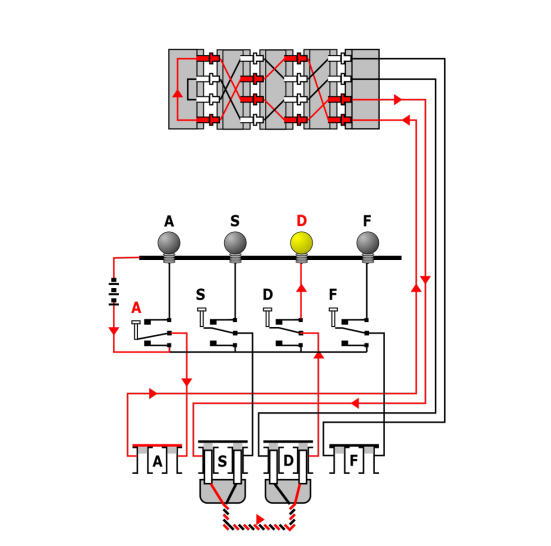
\includegraphics[scale = .9]{pathway.png}
    \caption{Pathway of Electrical Flow (a figure taken from the paper "A review on mathematical strength and analysis of Enigma"}
    \label{fig:path}
\end{figure}
\begin{figure}[h!]
    \centering
    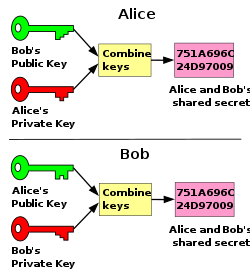
\includegraphics[scale = .7]{dh-graph.png}
    \caption{Diffie-Hellman Key Exchange (a figure taken from an article from Wikiwand)}
    \label{fig:dh}
\end{figure}
\begin{figure}[h!]
    \centering
    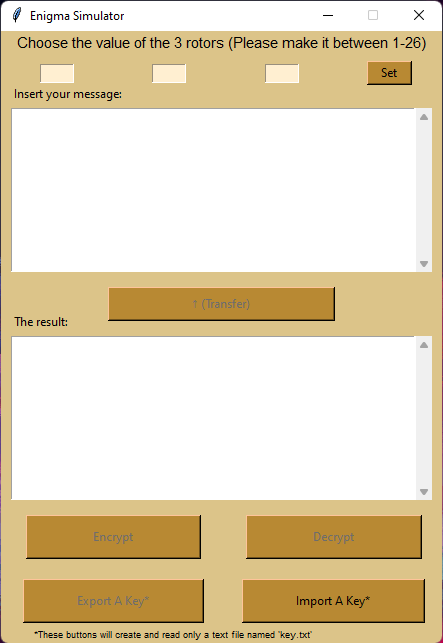
\includegraphics[scale = 0.8]{interface.png}
    \caption{Interface of the Enigma simulator}
    \label{fig:infac}
\end{figure}
\begin{figure}[h!]
    \centering
    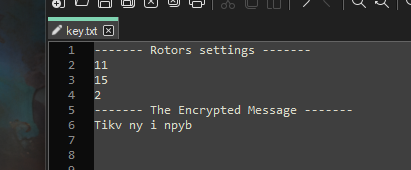
\includegraphics[scale = 0.8]{keysample.png}
    \caption{Contents of sample key.txt file (created during export)}
    \label{fig:sample}
\end{figure}

% that's all folks
\end{document}


